% !TEX root = ../main.tex
\chapter{Implementacja i~środowisko badawcze}
\label{chap:implementacja}

Rozdział dokumentuje implementację referencyjnej bramy pośredniczącej MCP~\cite{mcp_spec} (Python 3.12, FastMCP~\cite{fastmcp}, PostgreSQL 16 z~rozszerzeniem \texttt{pgvector}~\cite{pgvector}, Apache Kafka~\cite{kreps2011kafka} w~trybie KRaft) oraz aparaturę badawczą, odpowiadając na pytanie, jak fizycznie skonstruowano system i~środowisko eksperymentalne. Modele formalne opisano w~Rozdziale~\ref{chap:projekt}, a~wyniki pomiarów w~Rozdziale~\ref{chap:wyniki}.


%%%%%%%%%%%%%%%%%%%%%%%%%%%%%%%%%%%%%%%%%%%%%%%%%%%%%%%%%%%%%%%%%%%%%%%%%%%%%%%
\section{Architektura środowiska uruchomieniowego}
\label{sec:architektura_srodowiska}

Repozytorium zawiera dwie konfiguracje środowiska: deweloperską, opartą na kontenerach Docker i~Docker Compose (tabela~\ref{tab:parametry_kontenerow}), służącą do lokalnych testów, oraz natywną, w~której wykonano rundę pomiarową (tabela~\ref{tab:parametry_rundy}). Topologia środowiska obejmuje węzeł relacyjno-wektorowy PostgreSQL 16 z rozszerzeniem \texttt{pgvector}, rozproszony broker Apache Kafka działający w trybie KRaft, współdzielony segment pamięci operacyjnej (\texttt{/dev/shm}) dedykowany dla transferu obiektów binarnych poza pasmem oraz autorską bramę pośredniczącą FastMCP. Zestawienie składowych infrastruktury oraz ich kluczowe parametry konfiguracyjne podsumowano w tabeli~\ref{tab:parametry_kontenerow}.

\begin{table}[!htbp]
\centering
\small
\caption{Parametry konfiguracji deweloperskiej (kontenery Docker; nieużywana w~rundzie pomiarowej)}
\label{tab:parametry_kontenerow}
\begin{tabular}{p{2.8cm} p{3.8cm} p{8.0cm}}
\toprule
\textbf{Usługa kontenerowa} & \textbf{Obraz bazowy} & \textbf{Kluczowe parametry konfiguracyjne} \\
\midrule
PostgreSQL 16 & \texttt{pgvector/}\allowbreak\texttt{pgvector:pg16} & \texttt{shared\_buffers=1GB}, \texttt{work\_mem=32MB}, \texttt{max\_connections=200}, port 5432, rozszerzenie \texttt{vector} (HNSW, $d=384$, \texttt{vector\_cosine\_ops}) \\
\addlinespace
Apache Kafka & \texttt{apache/kafka:latest} & Tryb KRaft (\texttt{broker,controller}), 3 partycje fizyczne, quorum voter \texttt{localhost:9093}, listener \texttt{PLAINTEXT://:9092} \\
\addlinespace
Segment /dev/shm & Pamięć RAM hosta & POSIX Shared Memory: przekazanie danych binarnych poza ramką JSON-RPC, bez kodowania Base64 (jednokrotne kopiowanie do segmentu) \\
\addlinespace
Inicjalizacja danych & Python 3.12 & \texttt{generate\_enterprise\_schema.py} (1000 tabel, 20 tabel centralnych), \texttt{seed\_1m\_records.py} (1 mln rekordów) \\
\bottomrule
\end{tabular}
\end{table}

\begin{table}[!htbp]
\centering
\small
\caption{Środowisko rundy pomiarowej (odczytane automatycznie i~zapisane w~manifeście rundy, plik \texttt{environment.json})}
\label{tab:parametry_rundy}
\begin{tabular}{p{4.2cm} p{10.4cm}}
\toprule
\textbf{Element} & \textbf{Wartość} \\
\midrule
Sprzęt & \wynGpu{} (\wynGpuMem~GiB), \wynCpu{} (przydział: \wynVcpu~vCPU, \wynRam~GB RAM) \\
System i~oprogramowanie & Linux \wynKernel; Python \wynPython; uruchomienie natywne, bez kontenerów \\
PostgreSQL & \wynPg{} z~pgvector \wynPgvector; \texttt{shared\_buffers} = \wynPgSharedBuffers, \texttt{work\_mem} = \wynPgWorkMem, \texttt{max\_connections} = \wynPgMaxConn, \texttt{jit} = \texttt{\wynPgJit}, \texttt{max\_parallel\_workers\_per\_gather} = \wynPgParallel, \texttt{statement\_timeout} = \wynStmtTimeout \\
Pozostałe usługi & Apache Kafka \wynKafka; Ollama \wynOllama{} (modele \texttt{qwen2.5-coder:3b} i~\texttt{qwen2.5-coder:7b}) \\
\bottomrule
\end{tabular}
\end{table}

W~konfiguracji deweloperskiej węzeł bazodanowy (kontener \texttt{mcp\_postgres}) oparto na obrazie \texttt{pgvector:}\allowbreak\texttt{pg16} i~skonfigurowano parametry silnika:
\begin{itemize}
    \item \texttt{shared\_buffers=1GB}: bufor stron relacyjnych i~indeksowych, 25\% pamięci RAM węzła (4~GB), co ogranicza podwójne buforowanie z~pamięcią podręczną jądra;
    \item \texttt{work\_mem=32MB}: pamięć na sortowania i~tablice haszujące, pozwalająca wykonywać sortowania kursorowe w~RAM bez zrzutu na dysk;
    \item \texttt{max\_connections=200}: limit połączeń uwzględniający równoległe obciążanie bramy przez harness pomiarowy;
    \item \texttt{pgdata}: trwały wolumen blokowy izolujący operacje I/O bazy od warstwy nakładkowej kontenera.
\end{itemize}

Broker Apache Kafka (kontener \texttt{mcp\_kafka}) działa w~trybie KRaft, z~tematem \texttt{telemetry\_test} o~trzech partycjach (parametry w~tabeli~\ref{tab:parametry_kontenerow}). Konfiguracja kontenerowa służy do lokalnego uruchamiania bramy i~testów; runda pomiarowa, której wyniki przedstawia Rozdział~\ref{chap:wyniki}, została wykonana na instancji chmurowej bez kontenerów, z~usługami uruchomionymi natywnie i~parametrami odczytanymi automatycznie ze środowiska (podrozdział~\ref{subsec:wyniki_powtarzalnosc}).

W~celu weryfikacji algorytmów selekcji schematu na dużym schemacie zaimplementowano generator \texttt{testbed/init-scripts/}\allowbreak\texttt{generate\_enterprise\_schema.py}, powoływany automatycznie przy starcie bazy. Generator tworzy syntetyczny magazyn danych złożony z 1000 relacji SQL podzielonych równomiernie na 5 domen biznesowych: finanse (\texttt{finance}), gospodarka magazynowa (\texttt{inventory}), kadry i płace (\texttt{hr}), zarządzanie relacjami z klientami (\texttt{crm}) oraz telemetria przemysłowa (\texttt{telemetry}) -- po 200 tabel w każdej domenie (20 encji bazowych powiązanych z 10 kwalifikatorami operacyjnymi). Generator (deterministyczny, ziarno 42) wyznacza 20 centralnych tabel typu Hub (po 4 w~domenie, m.in. \texttt{finance\_ledger\_entries\_daily}, \texttt{crm\_client\_accounts\_enterprise}, \texttt{inventory\_purchase\_orders\_raw\_materials}, \texttt{telemetry\_host\_servers\_datacenter\_a}). Rozkład stopni uzyskanego grafu, odtworzony generatorem bez bazy (analiza wtórna, skrypt \texttt{o6\_stopnie\_grafu.py}; liczba węzłów i~krawędzi zgodna z~logiem rundy), przedstawia rysunek~\ref{fig:stopnie_grafu}: \wynOsixHubs{} tabel centralnych ma stopień \wynOsixHubMin--\wynOsixHubMax, a~pozostałe \wynOsixPeriph{} tabel stopień 1--\wynOsixPeriphMax{} (\wynOsixLeTwo\% tabel ma stopień nie większy niż 2). Graf nie ma więc rozkładu potęgowego właściwego sieciom bezskalowym, lecz strukturę gwiaździstą z~wyraźnymi węzłami centralnymi. Strukturę uzupełniają tabele mostkujące relacje typu $N:M$ (36 na domenę), tabele satelickie pierwszego poziomu (72 na domenę) oraz łańcuchy satelickie 2- i~3-poziomowe (88 na domenę).

\begin{figure}[htbp]
\centering
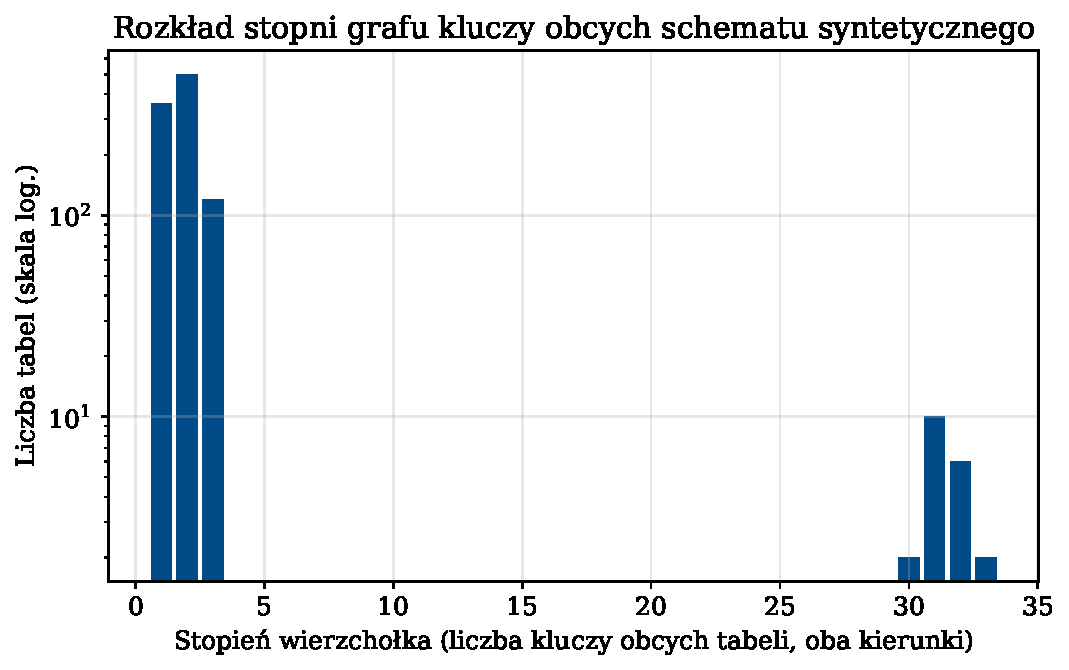
\includegraphics[width=0.75\linewidth]{rysunki/fig_stopnie_grafu.pdf}
\caption[Rozkład stopni grafu kluczy obcych schematu syntetycznego]{Rozkład stopni wierzchołków grafu kluczy obcych schematu syntetycznego (1000 tabel, 1174 klucze obce; analiza wtórna, generator deterministyczny)}
\label{fig:stopnie_grafu}
\end{figure}

Metadane relacyjne grafu bazy utrwalono w dedykowanej tabeli systemowej \texttt{public.}\allowbreak\texttt{schema\_foreign\_keys}, przechowującej 1174 zdefiniowane klucze obce wraz z powiązanymi kolumnami złączeń w formacie \texttt{JSONB} oraz indeksami B-drzewa na kolumnach \texttt{source\_table} i \texttt{target\_table}. Semantyczne opisy tabel umieszczono w relacji \texttt{public.schema\_embeddings}, w której kolumna \texttt{embedding} przechowuje gęste reprezentacje wektorowe o wymiarowości $d=384$, wygenerowane modelem \texttt{sentence-transformers/}\allowbreak\texttt{all-MiniLM-L6-v2}~\cite{reimers2019sentencebert}. Na kolumnie tej utworzono wielowarstwowy indeks grafowy HNSW~\cite{malkov2018hnsw} z operatorem odległości kosinusowej, gwarantujący logarytmiczną złożoność wyszukiwania najbliższych sąsiadów $\mathcal{O}(\log N)$.

Dla potrzeb ewaluacji paginacji kursorowej i transferu obiektów binarnych przygotowano relację \texttt{public.analytics\_orders}, zasilaną przez skrypt \texttt{seed\_1m\_records.py} wolumenem 1~000~000 rekordów przy użyciu binarnego strumieniowania \texttt{copy\_records\_to\_table} w paczkach po 25~000 wierszy. Tabela zawiera kolumny zróżnicowanych typów oraz kolumnę \texttt{document\_base64} o ładunkach 10--30~KB, wymuszającą w silniku PostgreSQL pozawierszowe przechowywanie atrybutów w strukturach TOAST (\emph{The Oversized-Attribute Storage Technique}). Do obsługi transferu OOB skonfigurowano współdzielony segment pamięci operacyjnej hosta podmontowany pod ścieżką \texttt{/dev/shm}.


%%%%%%%%%%%%%%%%%%%%%%%%%%%%%%%%%%%%%%%%%%%%%%%%%%%%%%%%%%%%%%%%%%%%%%%%%%%%%%%
\section{Implementacja autorskiego serwera MCP (Middleware Gateway)}
\label{sec:serwer_mcp}

Podstawowym komponentem warstwy pośredniczącej jest autorski serwer protokołu Model Context Protocol, zaimplementowany w module \texttt{src/mcp\_server/server.py}. Do budowy serwera wykorzystano framework FastMCP~\cite{fastmcp} w środowisku Python 3.12, w pełni zintegrowany z natywną pętlą zdarzeń \texttt{asyncio}. Komunikację z silnikiem PostgreSQL oparto na binarnym sterowniku \texttt{asyncpg}~\cite{asyncpg}, który realizuje protokół Frontend/Backend v3.0, omijając narzuty synchronicznego interfejsu DB-API 2.0 oraz biblioteki C \texttt{libpq}.

Zarządzanie połączeniami zrealizowano za pomocą asynchronicznej puli połączeń \texttt{asyncpg.Pool}, konfigurowanej w klasie \texttt{DatabaseConfig} (\texttt{min\_size=2}, \texttt{max\_size=10}), wyposażonej w procedurę rezerwowego uwierzytelniania środowiskowego. Cykl życia serwera kontrolowany jest przez asynchroniczny menedżer kontekstu \texttt{lifespan}. Odpowiada on za deterministyczne utworzenie puli połączeń bazodanowych, uruchomienie asynchronicznego konsumenta Kafka w tle oraz powołanie wieloprocesowej puli wykonawczej \texttt{ProcessPoolExecutor} z bezpiecznym kontekstem \texttt{forkserver} dla analizatora zapytań SQL. Podczas procedury zatrzymania menedżer gwarantuje sekwencyjne zatrzymanie konsumenta strumieniowego, zamknięcie procesów roboczych puli oraz zwolnienie wszystkich aktywnych połączeń bazodanowych.

Publiczny interfejs serwera (\texttt{src/mcp\_server/server.py}) realizuje kontrakt z~tabeli~\ref{tab:mcp_interface_contract}. Narzędzie \texttt{execute\_read\_only\_query} wykonuje walidację AST w~\texttt{SqlSanitizer}, wykonuje zapytanie i~hermetyzuje rekordy w~bloku \texttt{<untrusted\_db\_record>}; narzędzie \texttt{execute\_query\_paginated} realizuje paginację keyset (\texttt{pagination.py}) z~kontrolą indeksów (\texttt{IndexCatalogGuard}), opcjonalną migawką MVCC (\texttt{TransactionSnapshotManager}) i~estymatorem Welforda; narzędzie \texttt{search\_schema} wywołuje \texttt{SchemaEngine.}\allowbreak\texttt{discover\_schema\_}\allowbreak\texttt{with\_graph\_pruning}; narzędzie \texttt{retrieve\_out\_of\_band\_payload} odczytuje ładunek z~segmentu \texttt{/dev/shm} lub z~pliku magazynu obiektów i~weryfikuje skrót SHA-256. Anomalie telemetryczne odebrane z~Kafki przez konsumenta \texttt{aiokafka} są udostępniane jako zasoby \texttt{telemetry://latest\_anomaly} i~\texttt{telemetry://live\_stream} oraz narzędzie \texttt{get\_latest\_telemetry\_anomalies}, czyli odczytywane przez klienta na żądanie.

Framework FastMCP generuje z~adnotacji typów języka Python schemat JSON Schema parametrów każdego narzędzia i~waliduje argumenty wywołania przed uruchomieniem kodu narzędzia.


%%%%%%%%%%%%%%%%%%%%%%%%%%%%%%%%%%%%%%%%%%%%%%%%%%%%%%%%%%%%%%%%%%%%%%%%%%%%%%%
\section{Silnik semantycznego odkrywania schematu}
\label{sec:schema_discovery}

Implementację mechanizmu progresywnego odkrywania schematów relacyjnych w architekturze JIT zrealizowano w module \texttt{src/mcp\_server/schema\_engine.py} (klasa \texttt{SchemaEngine}), stanowiącym implementację założeń projektowych z podrozdziału~\ref{sec:projekt_schema_discovery}.

Klasa \texttt{SchemaEngine} integruje cztery strategie wyszukiwania tabel, których założenia formalne opisano w~podrozdziale~\ref{sec:projekt_schema_discovery}: leksykalną BM25 (\texttt{retrieve\_bm25}, biblioteka \texttt{rank\_bm25}, indeks budowany w~pamięci RAM z~nazw tabel, kolumn z~\texttt{information\_schema.columns} i~komentarzy biznesowych), gęstą (\texttt{retrieve\_dense}, model \texttt{all-MiniLM-L6-v2}, $d=384$, operator odległości kosinusowej \texttt{<=>} na indeksie HNSW tabeli \texttt{public.schema\_embeddings} obsługiwany przez \texttt{asyncpg}), hybrydową fuzję RRF (\texttt{retrieve\_hybrid\_rrf}, $k_{\text{RRF}} = 60$, równanie~\eqref{eq:rrf_formal}) oraz ekspansję grafową o~tabele mostkujące (\texttt{discover\_schema\_with\_graph\_pruning}), operujące na grafie NetworkX (\texttt{nx.DiGraph}) zbudowanym z~metadanych tabeli \texttt{public.schema\_foreign\_keys}.

Kod funkcji \texttt{discover\_schema\_with\_graph\_pruning}, wykrywającej tabele mostkujące na ścieżkach o długości $dist \le 2$ w grafie, zamieszczono na listingu~\ref{lst:graph_pruning} w załączniku~\ref{app:listingi}.

Wygenerowany zwarty blok DDL zawiera definicje kolumn, typów, kluczy głównych oraz explicite wyspecyfikowane klauzule relacji (\texttt{FOREIGN KEY ... REFERENCES}), co dostarcza modelowi językowemu niezbędny i nieskażony szumem kontekst relacyjny.


%%%%%%%%%%%%%%%%%%%%%%%%%%%%%%%%%%%%%%%%%%%%%%%%%%%%%%%%%%%%%%%%%%%%%%%%%%%%%%%
\section{Mechanizm adaptacyjnej paginacji kursorowej}
\label{sec:smart_pagination}

Paginację kursorową zaprojektowaną w~podrozdziale~\ref{sec:projekt_smart_pagination} (predykat keyset, kursor HMAC, migawka MVCC, estymator Welforda) zaimplementowano w~module \texttt{src/mcp\_server/pagination.py}, w~funkcjach \texttt{build\_keyset\_query} i~\texttt{fetch\_paginated\_data}. Rozbicie predykatu DNF na gałęzie \texttt{UNION ALL} włącza parametr \texttt{use\_union\_all} (domyślnie aktywny w~\texttt{fetch\_paginated\_data}). Moduł \texttt{IndexCatalogGuard} odpytuje widoki katalogowe (\texttt{pg\_indexes}, \texttt{pg\_am}, \texttt{pg\_class}, \texttt{pg\_attribute}) z~60-sekundowym buforem TTL, sprawdzając, czy kolumny sortowania tworzą lewostronny prefiks indeksu B-drzewa; przy jego braku dławi wielkość paczki do 50 wierszy, chroniąc \texttt{shared\_buffers} i~\texttt{work\_mem} przed skanem sekwencyjnym. Kod procedury zamieszczono na listingu~\ref{lst:keyset_pagination} w~załączniku~\ref{app:listingi}.


%%%%%%%%%%%%%%%%%%%%%%%%%%%%%%%%%%%%%%%%%%%%%%%%%%%%%%%%%%%%%%%%%%%%%%%%%%%%%%%
\section{Transfer danych binarnych Out-of-Band i asynchroniczne strumieniowanie}
\label{sec:transfer_binarny_strumieniowanie}

Fizyczną realizację mechanizmów transferu obiektów wielkich poza pasmem oraz asynchronicznego strumieniowania zdarzeń, sformalizowanych w podrozdziale~\ref{sec:projekt_oob}, wdrożono w modułach \texttt{src/mcp\_server/out\_of\_band.py} oraz \texttt{src/mcp\_server/streaming.py}.

Dyspozytor \texttt{DataTransferDispatcher} obsługuje tryby z~enumeracji \texttt{TransferMode}: \texttt{IN\_BAND} (Base64 w~ładunku JSON-RPC dla ładunków poniżej progu \texttt{threshold\_bytes = 64 KB}, stanowiącego zachowawczy próg startowy podlegający rekonfiguracji do progu zmierzonego dla danego środowiska; na jednym węźle wyniósł on \wynSstarLoopShm~KiB, podrozdział~\ref{sec:wyniki_scenariusz_b1}), \texttt{OOB\_POSIX\_SHM} (nazwany segment \texttt{multiprocessing.shared\_memory.SharedMemory} w~\texttt{/dev/shm}, skrót SHA-256 i~deskryptor JSON; aktywne segmenty są rejestrowane w~\texttt{\_ACTIVE\_SHM\_SEGMENTS} i~zwalniane procedurą \texttt{atexit}), \texttt{OOB\_HTTP\_STREAM} (jednorazowy adres URL z~podpisem HMAC-SHA256 i~czasem ważności \texttt{expires\_at}) oraz \texttt{AUTO} (kierowanie ładunków powyżej progu $S^*$ do pamięci współdzielonej). Stały narzut przygotowania deskryptora $\delta_{\text{OOB}}$ jest mierzony zegarem \texttt{time.perf\_counter\_ns()} i~dołączany do deskryptora.

W module \texttt{src/mcp\_server/streaming.py} zrealizowano asynchronicznego konsumenta komunikatów telemetrycznych w klasie \texttt{KafkaTelemetryConsumer}. Moduł bazuje na bibliotece \texttt{aiokafka} i~realizuje ciągły nasłuch tematu \texttt{telemetry\_test} w~asynchronicznej pętli \texttt{\_consume\_loop}. Odebranie komunikatu o statusie \texttt{CRITICAL\_ANOMALY} skutkuje natychmiastowym zapisem zdarzenia w~pamięci podręcznej (\texttt{deque(maxlen=100)}) oraz asynchronicznym wywołaniem zarejestrowanych funkcji zwrotnych subskrybentów SSE. Zastosowanie modelu sterowanego zdarzeniami eliminuje konieczność aktywnego odpytywania bazy przez agenta.


%%%%%%%%%%%%%%%%%%%%%%%%%%%%%%%%%%%%%%%%%%%%%%%%%%%%%%%%%%%%%%%%%%%%%%%%%%%%%%%
\section{Moduł bezpieczeństwa zapytań (SQL Sanitizer)}
\label{sec:bezpieczenstwo_zapytan}

Perymetr bezpieczeństwa zaprojektowany w~podrozdziale~\ref{sec:projekt_bezpieczenstwo} wdrożono w~module  \texttt{src/mcp\_server/security.py} (klasa \texttt{SqlSanitizer}) w~oparciu o~bibliotekę analizy składniowej \texttt{sqlglot}~\cite{sqlglot} i~dialekt \texttt{postgres}. Ponieważ budowa i~trawersowanie drzewa AST silnie obciążają procesor, walidację delegowano do puli \texttt{concurrent.futures.ProcessPoolExecutor} (funkcje \texttt{get\_process\_pool} i~\texttt{async\_validate\_query}) powoływanej z~kontekstem \texttt{forkserver}. Standardowy \texttt{fork} w~procesie wielowątkowym z~bibliotekami C (\texttt{sqlglot}, sterowniki binarne) grozi zakleszczeniem procesów potomnych na zduplikowanych muteksach, a~\texttt{spawn} generuje narzut zimnego startu interpretera; \texttt{forkserver} tworzy procesy robocze z~jednowątkowego procesu zarządczego, izolując pamięciowo pętlę \texttt{asyncio}.

Reguły walidacji z~podrozdziału~\ref{subsec:projekt_perymetr_ochronny} zrealizowano w~funkcjach \texttt{prevent\_multi\_statements}, \texttt{validate\_read\_only}, \texttt{enforce\_limit} (dopisanie lub redukcja klauzuli \texttt{LIMIT} do wartości maksymalnej, ochrona przed atakami Denial of Service) oraz \texttt{encapsulate\_untrusted\_database\_records}. Zbiór \texttt{FORBIDDEN\_AST\_NODES}, przeszukiwany rekurencyjnie w~całym drzewie (także w~klauzulach CTE), obejmuje węzły: \texttt{Insert}, \texttt{Update}, \texttt{Delete}, \texttt{Merge}, \texttt{Drop}, \texttt{Create}, \texttt{Alter}, \texttt{TruncateTable}, \texttt{Grant}, \texttt{Revoke}, \texttt{Copy}, \texttt{Command}, \texttt{Execute}, \texttt{Pragma}, \texttt{Into}, \texttt{Analyze}, \texttt{Set}, \texttt{Transaction}, \texttt{Commit} i~\texttt{Rollback}. Rekordy zwracane z~bazy są oczyszczane ze znaków specjalnych XML i~tokenów sterujących LLM (\texttt{<|im\_start|>}, \texttt{<|im\_end|>}, \texttt{[INST]}, \texttt{<<SYS>>}), a~następnie hermetyzowane w~bloku \texttt{<untrusted\_db\_record role="data\_only" execution\_forbidden="true">}, co ogranicza ryzyko ataków \emph{Second-Order Prompt Injection}.

Asynchroniczną delegację walidacji do puli \texttt{forkserver} przedstawiono na listingu~\ref{lst:ast_sanitizer} w załączniku~\ref{app:listingi}.

\paragraph{Deterministyczna weryfikacja poprawności w pakiecie testów jednostkowych.} Komponenty logiczne bramy -- estymator Welforda, mechanizm \texttt{IndexCatalogGuard}, kryptograficzny kursor HMAC oraz moduł migawek transakcyjnych MVCC -- stanowią integralne elementy architektury bramy. Ich niezmienniki algorytmiczne, deterministyczną poprawność oraz zachowanie w stanach brzegowych zweryfikowano w dedykowanym pakiecie testów jednostkowych (\texttt{tests/test\_mechanizmy\_bez\_ewaluacji.py}, \texttt{tests/test\_keyset\_nulls.py}). Testy te potwierdziły: odrzucenie kursora o naruszonej integralności lub niepoprawnym podpisie HMAC, bezpieczne ograniczenie rozmiaru paczki do 50 wierszy i odrzucenie zapytania w trybie ścisłym przy braku optymalnego indeksu B-drzewa, ścisłą zgodność estymacji wariancji i średniej algorytmem Welforda ze statystykami próbkowymi, a także poprawność generowania predykatu keyset w obecności wartości \texttt{NULL}.


%%%%%%%%%%%%%%%%%%%%%%%%%%%%%%%%%%%%%%%%%%%%%%%%%%%%%%%%%%%%%%%%%%%%%%%%%%%%%%%
\section{Klient agentowy oraz zautomatyzowana aparatura pomiarowa}
\label{sec:klient_aparatura}

W~celu przeprowadzenia powtarzalnych eksperymentów badawczych zaimplementowano klienta agentowego oraz modułowy runner pomiarowy. Klient agentowy oparto na paradygmacie ReAct~\cite{yao2023react}, zrealizowanym w klasie \texttt{ReActAgentLoop} (moduł \texttt{src/agent\_client/agent\_loop.py}). Pętla wykonawcza koordynuje sekwencję Myśl, Akcja oraz Obserwacja. Komunikację z serwerem FastMCP zaimplementowano w klasach \texttt{StdioMcpClient} (anonimowe potoki nienazwane \texttt{stdin}/\texttt{stdout}) oraz \texttt{SseMcpClient} (asynchroniczny transport HTTP/SSE).

W~aparaturze pomiarowej zdefiniowano dwa profile modeli językowych, obsługiwane przez serwer Ollama na akceleratorze GPU:
\begin{itemize}
    \item \textbf{Profil 3B:} model \texttt{qwen2.5-coder:3b};
    \item \textbf{Profil 7B:} model \texttt{qwen2.5-coder:7b}.
\end{itemize}
Oba profile używają temperatury $T = 0$, stałego ziarna, limitu 1024 tokenów wyjściowych i~okna kontekstu \texttt{num\_ctx} = \wynNumCtx; liczby tokenów promptu i~odpowiedzi oraz powód zakończenia generacji są odczytywane z~liczników serwera Ollama, co pozwala wykryć obcięcie kontekstu lub odpowiedzi. Profile różnią się wyłącznie modelem.

Fundament aparatury pomiarowej stanowi klasa \texttt{BenchmarkHarness} zlokalizowana w module \texttt{benchmarks/harness.py}. Konstrukcja runnera pomiarowego opiera się na następujących zasadach metodologicznych:
\begin{itemize}
    \item \textbf{Determinizm środowiska bazodanowego:} Przed każdym zapytaniem pomiarowym sesja bazy danych jest resetowana poleceniem \texttt{DISCARD ALL}, które czyści pamięć podręczną planów zapytań, blokady oraz ustawienia sesji. Wszystkie generatory liczb losowych (zapytania, wektory, bootstrap, model) używają stałych ziaren zapisanych w~pliku konfiguracji rundy;
    \item \textbf{Biegi rozgrzewkowe:} Punkty pomiarowe poprzedzane są nieewaluowanymi przebiegami rozgrzewkowymi, których liczbę określa konfiguracja scenariusza (np. 2 dla paginacji, 5 dla transferu OOB, 5~s dla każdego poziomu obciążenia współbieżnego);
    \item \textbf{Sztywny limit czasu zapytań:} W konfiguracji puli połączeń \texttt{asyncpg} wymuszono limit \texttt{statement\_timeout = '10000ms'}, zapobiegający blokowaniu aparatury przez kwerendy zawieszające transakcje pod obciążeniem;
    \item \textbf{Wysokorozdzielcza aparatura próbkowania czasu:} Pomiar czasu wykonania operacji realizowany jest nanosekundowym zegarem monotonicznym \texttt{time.perf\_counter\_ns()};
    \item \textbf{Asynchroniczny próbnik opóźnienia pętli zdarzeń (\texttt{EventLoopLagProbe}):} W scenariuszach współbieżnych uruchamiana jest sonda w tle, która co 10~ms próbuje wybudzić się z uśpienia (\texttt{asyncio.sleep(0.010)}). Różnica pomiędzy czasem rzeczywistym a oczekiwanym wyznacza bezpośrednio opóźnienie harmonogramu (\emph{timer drift}) wywołane blokowaniem pętli zdarzeń;
    \item \textbf{Deterministyczna tokenometria:} Zliczanie tokenów generowanych w ładunkach realizowane jest biblioteką \texttt{tiktoken} (enkoder \texttt{cl100k\_base});
    \item \textbf{Profilowanie zasobów systemowych:} Pamięć mierzona jest jako suma PSS (\emph{Proportional Set Size}) procesu serwera i~wszystkich jego procesów potomnych za pomocą biblioteki \texttt{psutil}, co pozwala uwzględnić koszt puli procesów bez wielokrotnego liczenia stron współdzielonych;
    \item \textbf{Ustrukturyzowany zapis danych surowych:} Wszystkie zarejestrowane próbki czasowe, metadane i wskaźniki są serializowane do kolumnowych plików Apache Parquet oraz tabelarycznych CSV w~katalogu wyników rundy, a~manifest rundy zapisuje wersję kodu, konfigurację, ziarna, opis środowiska, skróty wag modeli oraz sumy kontrolne SHA-256 wszystkich plików wynikowych.
\end{itemize}

Zestaw scenariuszy badawczych uruchamianych w~jednej rundzie pomiarowej obejmuje m.in. scenariusze wymienione w~tabeli~\ref{tab:aparatura_pomiarowa}. Ich charakterystykę inżynierską, badane mechanizmy, wielkości prób oraz aparaturę wnioskowania statystycznego zestawiono w tabeli~\ref{tab:aparatura_pomiarowa}.

\begin{table}[!htbp]
\centering
\footnotesize
\setlength{\tabcolsep}{3pt}
\caption{Zestawienie scenariuszy badawczych, aparatury pomiarowej oraz metod weryfikacji statystycznej}
\label{tab:aparatura_pomiarowa}
\begin{tabular}{>{\raggedright\arraybackslash}p{2.5cm} >{\raggedright\arraybackslash}p{3.8cm} >{\raggedright\arraybackslash}p{1.7cm} >{\raggedright\arraybackslash}p{3.7cm} >{\raggedright\arraybackslash}p{2.5cm}}
\toprule
\textbf{Skrypt / Scenariusz} & \textbf{Badany mechanizm i cel} & \textbf{Wielkość próby} & \textbf{Rejestrowane metryki surowe} & \textbf{Weryfikacja statystyczna} \\
\midrule
\texttt{bench\_schema\_}\allowbreak\texttt{quality.py} & Selekcja schematu, ekspansja grafowa o~tabele mostkujące, Text-to-SQL na dwóch profilach modeli & $N=500$ zapytań (150 prostych, 250 średnich, 100 złożonych) & Recall i~Precision (tabele i~kolumny), Valid SQL, Execution Accuracy, liczniki tokenów, kategorie błędów & Test Wilcoxona, dokładny test McNemara, 95\% CI Cloppera--Pearsona \\
\addlinespace
\texttt{bench\_ttft\_}\allowbreak\texttt{scaling.py} & Czas do pierwszego tokenu w~funkcji rozmiaru promptu & 6 rozmiarów promptu $\times$ 30 powtórzeń $\times$ 2 profile & $TTFT$, czas całkowity, \texttt{prompt\_eval\_count} & Regresja liniowa, bootstrap 95\% CI \\
\addlinespace
\texttt{bench\_pagination\_}\allowbreak\texttt{advanced.py} & Paginacja keyset, OFFSET i~bez indeksu; postać predykatu & 10 offsetów $\times$ 10 powtórzeń & Opóźnienie strony, plany \texttt{EXPLAIN}, spójność sekwencji & Regresja liniowa, mediana i~zakres \\
\addlinespace
\texttt{bench\_oob\_}\allowbreak\texttt{crossover.py} & Dyspozytor danych OOB, punkt przecięcia $S^*(\text{RTT})$ dla In-Band, SHM i HTTP & 9 rozmiarów 512~B -- 50~MiB $\times$ 50 powtórzeń, 3 profile sieci & Czas transferu End-to-End i~jego składowe, objętość ramki, integralność SHA-256 & Test Manna--Whitneya, bootstrap 95\% CI progu $S^*$ \\
\addlinespace
\texttt{bench\_schema\_}\allowbreak\texttt{drift.py} & Odporność na dynamiczny dryf schematu podczas współbieżnych migracji DDL & 50 nowych relacji, 50 kluczy FK, kwerendy w toku & Czasy składowych przeładowania metadanych, opóźnienie i~błędy zapytań w~trakcie dryfu & Analiza percentyli \\
\addlinespace
\texttt{bench\_}\allowbreak\texttt{concurrency}\allowbreak\texttt{.py} & Wydajność i skalowalność pętli zdarzeń pod obciążeniem (SYNC, THREAD, POOL) & $M \le 500$ ($M \in \{1, 5,$ \newline $10, 25, 50,$ \newline $100, 500\}$) & Przepustowość (RPS), opóźnienie odpowiedzi, opóźnienie pętli zdarzeń, suma PSS drzewa procesów & Test Manna--Whitneya, bootstrap 95\% CI różnicy median, percentyle \\
\addlinespace
\texttt{bench\_security\_}\allowbreak\texttt{suite.py} & Odporność zapory AST i guardrails na wektory SQLi oraz Prompt Injection & \wynSecTotal{} unikalnych wektorów & FPR, AMR, odsetek przepuszczonych \texttt{SELECT} z~efektami ubocznymi, odsetek rekordów z~pozostałymi tokenami sterującymi, odpowiedzi modelu na wektory wstrzykiwania & 95\% CI Cloppera--Pearsona, dokładny test McNemara \\
\addlinespace
\texttt{statistical\_}\allowbreak\texttt{analysis.py} & Formalna weryfikacja hipotez badawczych z surowych wektorów pomiarowych & Zbiorcze wektory z plików Parquet & Statystyki testowe, wartości $p$, wielkość efektu $r$, przedziały ufności & Testy Wilcoxona, McNemara i~Manna--Whitneya, bootstrap \\
\bottomrule
\end{tabular}
\end{table}

Zaprojektowane środowisko testowe, zunifikowana brama pośrednicząca FastMCP oraz zautomatyzowana aparatura pomiarowa posłużyły do przeprowadzenia pełnego pakietu ewaluacji empirycznej, której szczegółowe wyniki ilościowe, analiza statystyczna oraz interpretacja efektywnościowa stanowią treść Rozdziału~\ref{chap:wyniki}.
